\documentclass[11pt, conference]{IEEEtran}
\usepackage[spanish]{babel}
\usepackage[utf8]{inputenc}
\usepackage{amsmath}
\usepackage{amsfonts}
\usepackage{cite}
\usepackage{graphicx}

\begin{document}
\title{\bf Algoritmos de Criptografía}
\author{Jose David Mamani Vilca\\
	Kevin Jhomar Sanchez Sanchez\\
	Percy Maldonado Quispe\\
	Luis Fernando Ttito Surco\\
	Angel Cutipa Samayani
	}
\maketitle
%\tableofcontents 
%\maketitle
%\listoffigures

\section{\bf ¿Qué es la criptografía?}

\subsection{\bf Criptografia Cuantica}
\subsubsection{\bf Mecanica Cuantica en Criptografia}

\begin{itemize}
\item Principio de Incertidumbre. 
\item Polarizacion de un Foton.
\item Qubits.
\item Verschrankung
\item Teorema de no-clonacion.
\end{itemize} 

\subsubsection{\bf Distribucion de Claves Cuanticas}
Se deben cumplir las siguientes condiciones:

\begin{itemize}
\item Ningun intruso puede obtener la clave transmitida 
\item Cualquier intento de intromisión para obtener la clave transmitida puede ser detectado con alta probabilidad
\item Los usuarios pueden estar seguros de que están compartiendo la misma clave
\end{itemize}

\subsubsection{\bf Protocolo BB84}
El esquema propuesto en 1984 por Brassard y Bennett implica el envío de fotones preparados en diferentes estados de polarización.
\begin{figure}[hbtp]
\centering
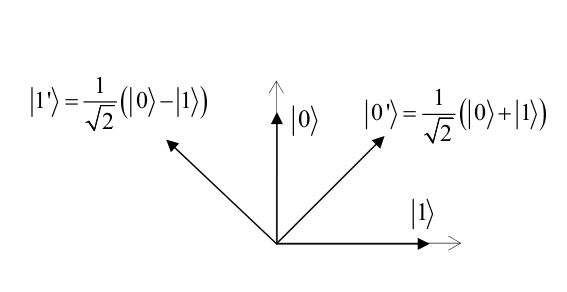
\includegraphics[scale=0.4]{1.png} 
\caption{Representacion de la polarizacion de fotones
en el protocolo BB84}
\end{figure}
Usando un filtro de polarización, se selecciona el ángulo de polarización con respecto a la horizontal. Los fotones polarizados $\leftrightarrow \nearrow$ representan el binario 0, los fotones polarizados $\updownarrow \searrow$ representan el binario 1; entonces una secuencia de bits puede ser convertida en una secuencia de fotones polarizados.

{\bf 1. Sin la Presencia de Eve.- }
\begin{itemize}
\item Alicia codifica bits como fotones polarizados. La primera fila indica la secuencia de bits. La segunda indica la orientación usada por el filtro. La tercera indica el resultado de la polarización.

\begin{figure}[hbtp]
\centering
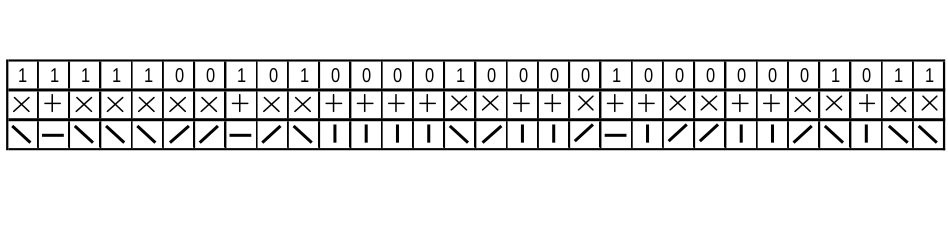
\includegraphics[scale=0.22]{2.png} 
\caption{Alice codifica bits como fotones polarizados}
\end{figure}

Alicia genera una secuencia de fotones. Cuando Bob recibe los fotones, decide aleatoriamente si medir las polarizaciones a lo largo de las direcciones rectilíneas o a lo largo de las diagonales. De esta forma Bob podría extraer un bit de información por cada fotón.

\item Bob decodifica fotones polarizados como bits. La primera fila indica la secuencia de fotones recibida. La segunda fila indica la configuración del cristal de calcita de Bob. La tercera fila indica el resultado de la medición.

\begin{figure}[hbtp]
\centering
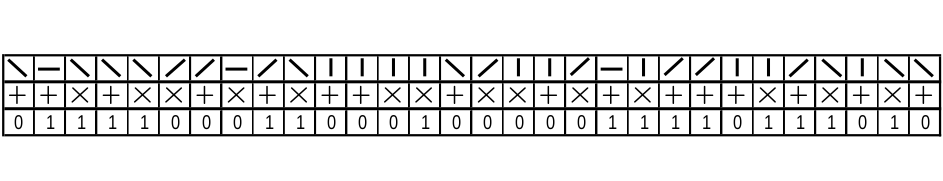
\includegraphics[scale=0.22]{3.png} 
\caption{Bob decodifica fotones polarizados como bits}
\end{figure}

Este comportamiento se explica por el principio de incertidumbre de Heisenberg.
\begin{figure}[hbtp]
\centering
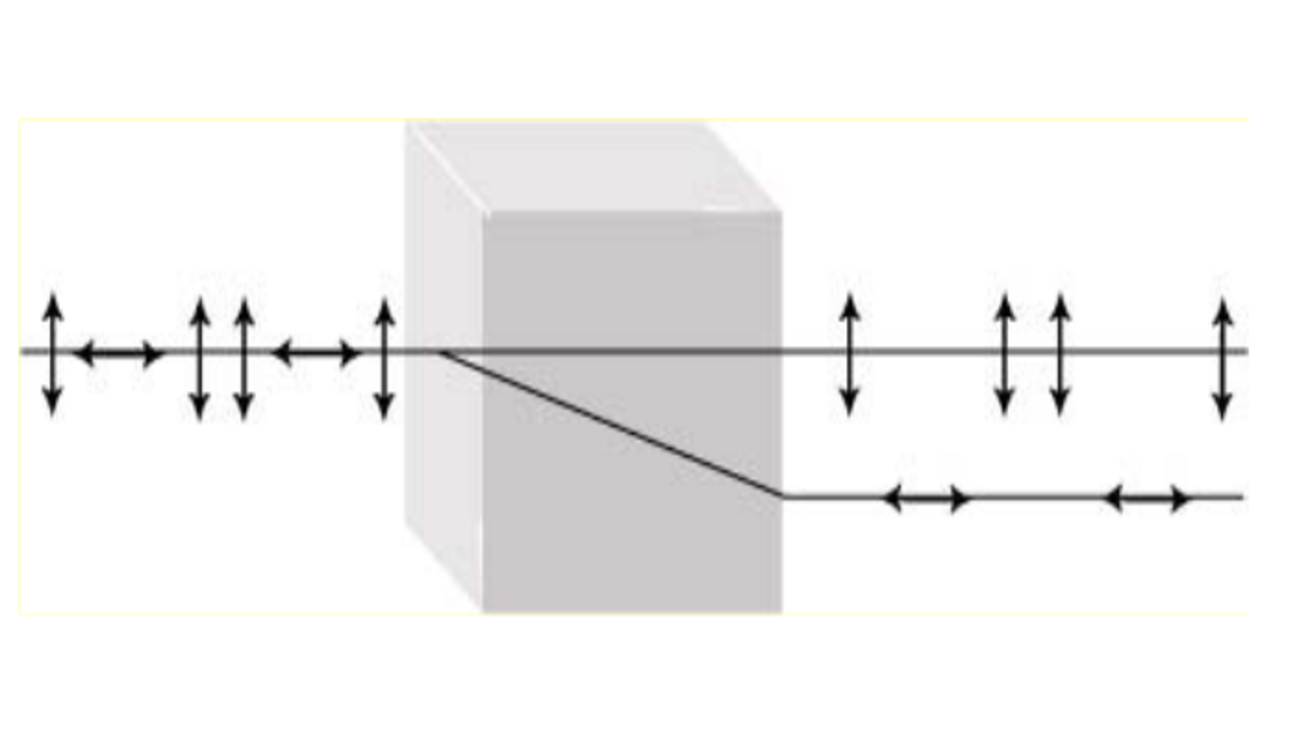
\includegraphics[scale=0.15]{4.png} 
\caption{Cristal de Calcita que separa fotones de diferente polarización}
\end{figure}

Alicia le dice a Bob (canal clasico) el valor de los bits que debió haber medido, y la verificación debe asegurar que los bits de Bob concuerdan al 100\% con los de Alicia.

La probabilidad de detectar un espía que esté presente es $1-\left(\frac{3}{4}\right)^{N}$.

\item Alicia y Bob comparan un subgrupo de bits para probar, y verificar la presencia de un espía. En todos los bits se usó la misma orientación para polarizar y medir, y el valor del bit es igual, mostrando que no hay un espía presente.

\begin{figure}[hbtp]
\centering
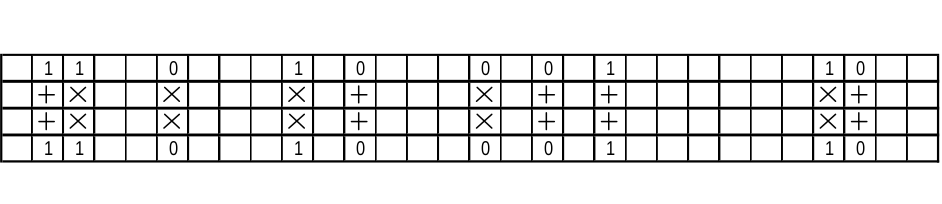
\includegraphics[scale=0.22]{5.png} 
\caption{Alicia y Bob comparan un subgrupo de bits}
\end{figure}

\item Clave generada. Los casos en que la orientación del polarizador es igual a la orientación del cristal, se representan por :), y esto significa que el bit se tomó como parte de la clave.

\begin{figure}[hbtp]
\centering
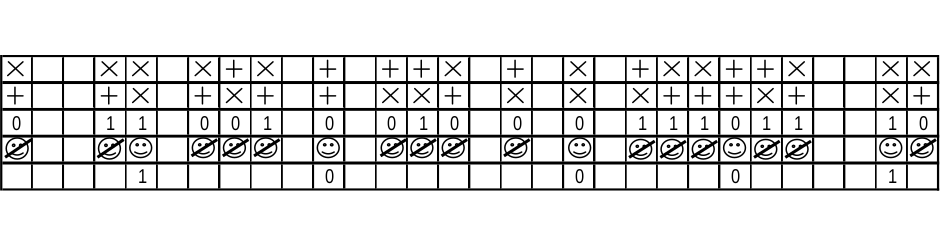
\includegraphics[scale=0.22]{6.png} 
\caption{Clave Generada}
\end{figure}

\end{itemize}

{\bf 2. Eve Presente.- } En este caso, para que Eva pueda medir los fotones interceptados, debe haber escogido una orientación de polarización. Si Eva quisiera tener certeza de no ser detectada, necesitaría correr la suerte de escoger para cada bit transmitido la misma orientación de polarización que Alicia, lo cual, si el tamaño de la clave es lo suficientemente largo, sería prácticamente imposible. Si Eva elige la orientación incorrecta, modificará la polarización del fotón y su presencia podrá ser detectada en la fase de prueba.

\begin{itemize}
\item Codificación de los bits de Alicia a estados de polarización:

\begin{figure}[hbtp]
\centering
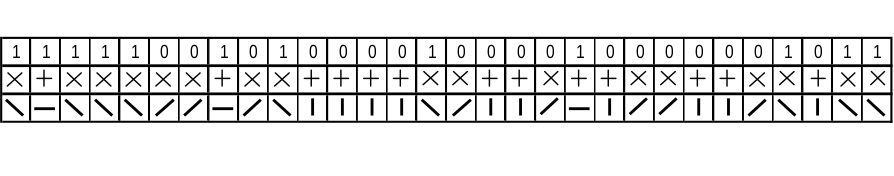
\includegraphics[scale=0.22]{7.png} 
\caption{Codificación de los bits de Alicia}
\end{figure}
\item Intercepción y medición de Eva (Si las polarizaciones no son iguales, Eva modifica irreparablemente el estado original):

\begin{figure}[hbtp]
\centering
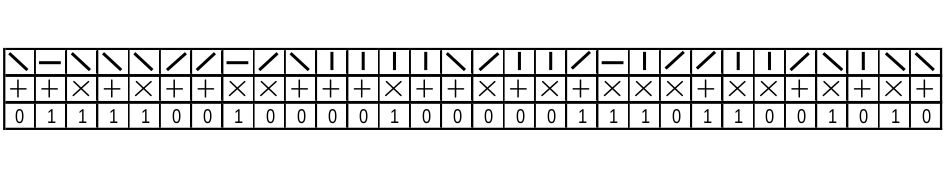
\includegraphics[scale=0.22]{8.png} 
\caption{Intercepción y medición de Eva}
\end{figure}

\item Bob, aún sin estar consciente de la presencia de Eva, realiza sus mediciones:

\begin{figure}[hbtp]
\centering
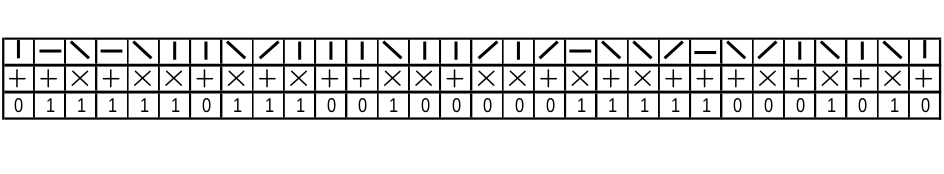
\includegraphics[scale=0.22]{9.png} 
\caption{Bob realiza mediciones}
\end{figure}

\item Pero en la fase de prueba, Alicia y Bob detectan la presencia de Eva y deciden desechar toda la secuencia de fotones para empezar de nuevo el procedimiento.

\begin{figure}[hbtp]
\centering
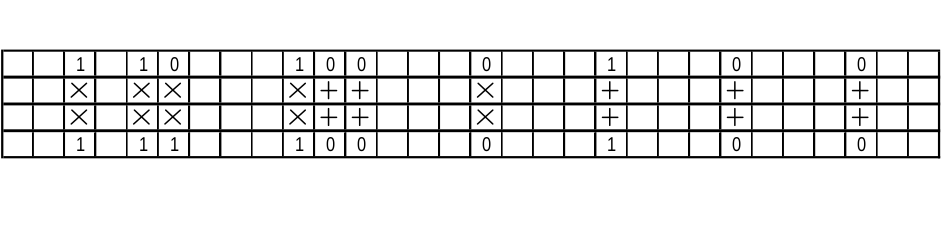
\includegraphics[scale=0.22]{10.png} 
\caption{Detectan la presencia de Eva}
\end{figure}
\end{itemize}

\subsubsection{\bf Conclusiones}
La seguridad de la criptografía cuántica descansa en las bases de la mecánica cuántica, a diferencia de la criptografía de clave pública tradicional la cual descansa en supuestos de complejidad computacional no demostrada de ciertas funciones matemáticas

\end{document}
